\section{Durchführung}
\label{sec:Durchführung}

Für die Messungen werden jeweils die gleichen Kathodenstrahlröhren genutzt.

\subsection{Messungen im E-Feld}

    Zuerst wird der Zusammenhang zwischen der Ablenkspannung und der Leuchtfleckverschiebung auf dem Schirm untersucht. Dafür werden für 5 verschiedene 
    Beschleunigungsspannungen $U_{\text{B}}$ im Bereich von $\SI{180}{\volt} - \SI{500}{\volt}$ der Leuchtfleck auf die 9 äquidistanten Punkte des 
    Leuchtschirms gebracht und dann die jeweilige Ablenkspannung $U_{\text{d}}$ notiert. Diese wird auf einem Voltmeter abgelesen.

    \begin{figure}[H]
        \centering
        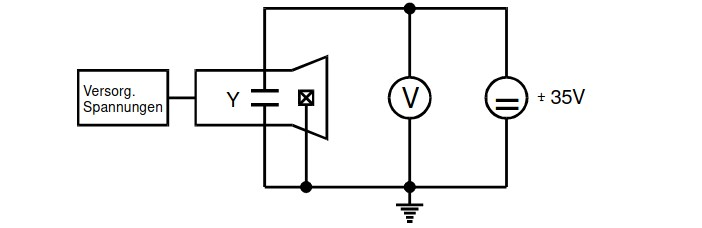
\includegraphics[width=0.6\textwidth]{bilder/messung_leuchtfleckverschiebung.jpg}
        \caption{Eine Schaltung zur Messung der Leuchtfleckverschiebung \cite{anleitung501}.}
        \label{fig:leuchtfleckverschiebung}
    \end{figure}

    \noindent Anschließend wird ein Kathodenstrahl-Oszillograph nach der Schaltung in \autoref{fig:kathodenstrahlosz_prinzip} aufgebaut. 
    An der x-Ablenkung ist die Sägezahnspannung und an der y-Ablenkung eine auszumessende Sinusspannung angelegt. Nun wird die Frequenz der
    Sägezahnspannung so verändert, dass sich auf dem Schirm stehende Bilder von einer halber, einer ganzen, zwei und drei Perioden der Sinusspannung
    zu sehen ist. Für diese Verhältnisse wird die Frequenz notiert.

    \begin{figure}[H]
        \centering
        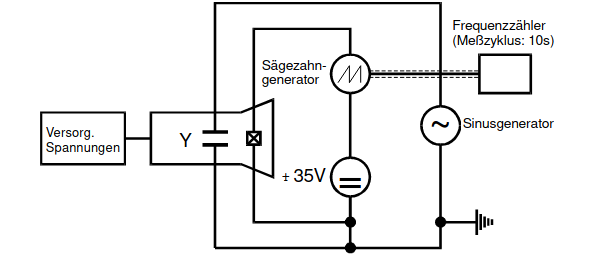
\includegraphics[width=0.6\textwidth]{bilder/prinzipschaltbild_kathodenstrahl.png}
        \caption{Prinzipschaltbild eines Kathodenstrahl-Oszillographen \cite{anleitung501}.}
        \label{fig:kathodenstrahlosz_prinzip}
    \end{figure}

    \begin{figure}[H]
        \centering
        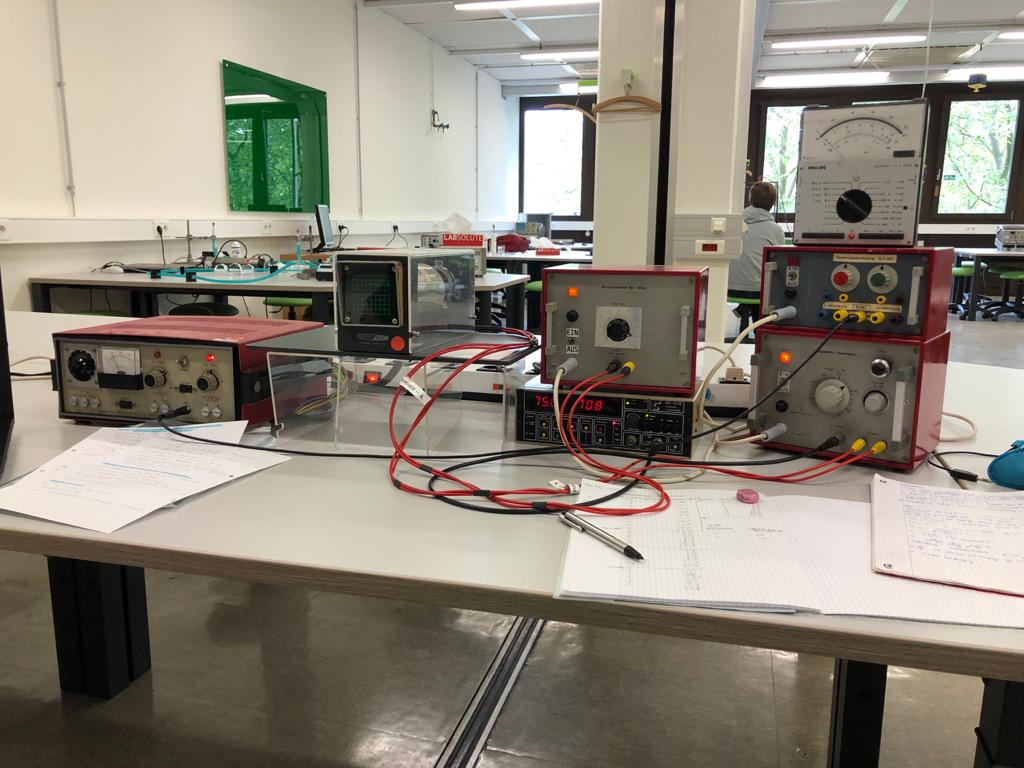
\includegraphics[width=0.6\textwidth]{bilder/foto_elektrisch.jpeg}
        \caption{Aufbau des Experimentes für die Messung mit einem elektrischen Feld.}
        \label{fig:aufbau_efeld}
    \end{figure} 

    \noindent In der \autoref{fig:aufbau_efeld} ist von links nach rechts ist die Beschaltung der Kathodenstrahlröhre, die Kathodenstrahlröhre, der Sinusgenerator auf dem 
    Frequenzzähler und das Voltmeter auf dem Gleichspannungsgenerator auf dem Sägezahngenerator zu sehen.

\subsection{Messung im B-Feld}

    Es wird ein Magnetfeld mit einem Helmholtzspulenpaar erzeugt; die Flussdichte $B$ ist im Mittelpunkt gegeben durch 
    \begin{equation*}
        \mu_0 \frac{8}{\sqrt{125}} \frac{N I}{R},
    \end{equation*}
    wobei $N$ die Windungszahl, $R$ der Spulenradius und $I$ der Spulenstrom ist. Die Kathodenstrahlröhre wird zu Beginn nicht in Richtung der Horizontkomponente
    des Erdmagnetfeldes gelegt, da dies kaum einen Einfluss auf die Messung der spezifischen Ladung hat. Hierzu wird für zwei verschiedene Beschleunigungsspannungen 
    $U_{\text{B}} = \SI{250}{\volt}$ und $U_{\text{B}} = \SI{500}{\volt}$ der Leuchtfleck mit Hilfe eines elektrischen Feldes auf die oberste oder die unterste der
    äquidistanten Linien gelegt. Analog zur Messung der Leuchtfleckverschiebung wird der Leuchtfleck auf eine der äquidistanten Linien gebracht und der dafür benötigte
    Spulenstrom notiert. \\

    \noindent Abschließend wird die Intensität des lokalen Erdmagnetfeldes gemessen. Dazu wird die Position des Leuchtfleck in Nord-Süd-Ausrichtung der 
    Kathodenstrahlröhre notiert oder mit einem elektrischen Feld auf den Mittelpunkt des Schirms gelegt. Dann wird die Röhre in Ost-West-Richtung gedreht, sodass
    sich der Leuchtfleck verschiebt. Dann wird der Leuchtfleck durch das Magnetfeld des Helmholtzspulenpaar wieder auf den Ursprungsort gelegt und der 
    dafür benötigte Spulenstrom notiert. \\

    \noindent In der \autoref{fig:aufbau_bfeld} ist der Aufbau des Experimentes mit einem Magnetfeld zu sehen. Das Helmholtzspulenpaar ist auf einer drehbaren
    Platte gelagert, in seinem Mittelpunkt befindet sich die Kathodenstrahlröhre. Rechts daneben befindet sich das Amperemeter mit dem der Strom notiert wird und 
    daneben der Gleichspannungsgenerator auf der Beschaltung für die Kathodenstrahlröhre. 

    \begin{figure}[H]
        \centering
        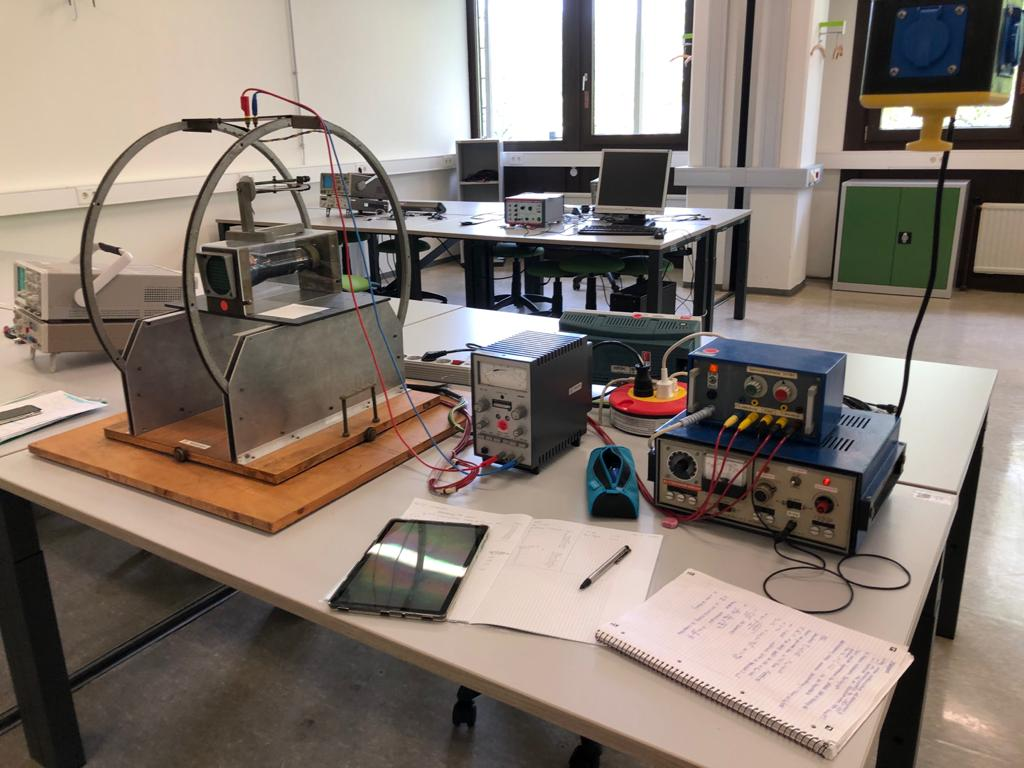
\includegraphics[width=0.6\textwidth]{bilder/foto_magnet.jpeg}
        \caption{Aufbau des Experimentes zur Messung mit einem Magnetfeld.}
        \label{fig:aufbau_bfeld}
    \end{figure} 


